\documentclass[11pt]{article}
\pdfoutput=1
\usepackage{simplemargins}
\usepackage{url}
\usepackage[pdftex]{graphicx}
\usepackage{setspace}
\graphicspath{{figures/}}
\usepackage{siunitx}
\setlength{\parindent}{0pt} 
\setlength{\parskip}{1.6ex} 
\setallmargins{1in} 
\linespread{1.6}
\usepackage[round]{natbib}
\usepackage{color}
\usepackage{subfigure}
\usepackage{booktabs}
\usepackage{pdflscape}
\usepackage[colorlinks=false,breaklinks]{hyperref}
\listfiles

% make subfigure labels capitalized
\renewcommand{\thesubfigure}{(\Alph{subfigure})}

%setup supplement
\newcommand{\beginsupplement}{%
        \setcounter{table}{0}
        \renewcommand{\thetable}{S\arabic{table}}
        \setcounter{figure}{0}
        \renewcommand{\thefigure}{S\arabic{figure}}
        \renewcommand{\thesection}{S\arabic{section}}
        \renewcommand{\thesubsection}{S\arabic{subsection}} 
     }

\begin{document}

% Title must be 150 characters or less
\begin{flushleft} 
\singlespacing
{\Large \textbf{The genetic architecture of local adaptation I: The genomic landscape of 
foxtail pine (\textit{Pinus balfouriana} Grev.\ \& Balf.) as revealed from a high-density linkage map}}
% Insert Author names, affiliations and corresponding author email.


Christopher J.\ Friedline$^{1}$, 
Brandon M. Lind$^{1}$,
Erin M. Hobson,$^{1}$,
Douglas E. Harwood$^{1}$, 
Annette Delfino Mix$^{2}$,
Patricia E. Maloney$^{3}$, and
Andrew J. Eckert$^{1,4}$


\bf{1} Department of Biology, Virginia Commonwealth University, Richmond, VA 23284
\\
\bf{2} Institute of Forest Genetics, USDA Pacific Southwest Research Station, Placerville, 
CA 95667
\\
\bf{3} Department of Plant Pathology, University of California, Davis, CA 95616
\\
\bf{4} Author for Correspondence


$\ast$ E-mail: aeckert2@vcu.edu
\end{flushleft}

\section*{Abstract}

Explaining the origin and evolutionary dynamics of the genetic architecture of adaptation
is a major research goal of evolutionary genetics.
Despite the controversy surrounding the success of the attempts to accomplish this goal, a full understanding of adaptive genetic variation 
necessitates knowledge about the genomic location and distributional patterns of the genetic components affecting fitness-related
phenotypic traits. Even with advancements to next generation sequencing technologies, the production of full
genome sequences for non-model species is often cost prohibitive, especially for tree species such as pines where genome
size often exceeds $20$ to $30$ Gbp in size. Here, we address this need by constructing a dense linkage map for 
foxtail pine (\textit{Pinus balfouriana} Grev. \& Balf.), with the ultimate goal of uncovering and explaining the origin
and evolutionary dynamics of adaptive genetic variation for drought tolerance in natural populations of this forest 
tree species. We utilized megagametophyte  arrays (\textit{n} $= 76 - 95$/tree) from four maternal trees in combination 
with double-digestion restriction site associated DNA sequencing (ddRADSeq) to produce a consensus linkage map covering $98.58\%$ 
of the foxtail pine genome, which was estimated to be $1276$ cM in length ($95\%$ CI: $1174-1378$ cM). A novel bioinformatic approach using iterative rounds 
of marker ordering and imputation was employed to produce single-tree linkage maps ($507 - 17066$ contigs/map).
These linkage maps were strongly collinear across maternal trees, with highly correlated marker orderings (Spearman's $\rho > 0.95$).
A consensus linkage map derived from these single-tree linkage maps contained $20655$ contigs divided into $12$ 
linkage groups along which $901$ unique positions were non-randomly distributed
with an average spacing of $1.34$ cM between adjacent positions (\textit{n}$ = 23$ contigs/position). Of the $20655$ contigs positioned on the consensus 
linkage map, $5627$ had enough sequence similarity to contigs contained within the most recent build of the loblolly pine 
(\textit{P. taeda} L.) genome to identify them as  putative homologs containing both genic and non-genic loci. Importantly,
all $901$ unique positions on the consensus linkage map had at least one contig with putative homology to loblolly pine.
Our results indicate that high density linkage maps can be produced efficiently for non-model forest tree species 
and that these maps have important functions as community-wide resources and as tools with which to 
test hypotheses about the genetic architecture of adaptation. 

\textbf{Key words:} Adaptation, double-digestion restriction site associated DNA sequencing, foxtail pine, linkage mapping, 
\textit{Pinus balfouriana}

\section*{Introduction}

Evidence for adaptive evolution among populations of plants is commonly documented at both the phenotypic 
and molecular levels \citep{Kawecki:2004, Pannell:2013}, so that some of the best
examples of adaptive evolution within lineages come from the field of plant genetics \citep[e.g.,][]{Antonovics:1970}. 
Despite this evidence, relatively little work has focused explicitly on the genomic organization of loci contributing
to these patterns \citep{Hoffman:2008}, which likely stemmed from the lack of genomic resources for plants relative to animals.
Adaptive evolution has been extensively documented for forest trees, especially conifers, with many instances of 
local adaptation clearly being documented over the past century \citep{White:2007, Neale:2011}. Despite great advances 
in experimental technology, empirical focus has remained almost fully on the number, effect size, type, and interactions 
among loci contributing to adaptive evolution \citep{Neale:2011, Alberto:2013}.  A thorough examination of the 
genetic architecture of fitness-related traits, however, should also include 
an examination of the genomic organization of the loci contributing to trait variation. Here, we leverage 
this idea in the first of a series of papers dissecting the genetic architecture of fitness-related 
traits in a non-model conifer species, foxtail pine (\textit{Pinus balfouriana} Grev. \& Balf.), with the 
ultimate goal of testing explicit evolutionary hypotheses about the genomic organization of loci 
contributing to variation in fitness-related traits.

Ideally, the genomic organization of loci contributing to variation in fitness-related traits would follow 
naturally from the production of a genome sequence (i.e., a physical map). For many taxa, especially those with 
small to modest genome sizes, this is monetarily and computationally feasible using next-generation DNA sequencing 
technologies \citep{Koboldt:2013}. For taxa with large or complex genomes, however, even the advent of next generation DNA 
sequencing does not solve the complexity and cost hurdles associated with the production of a finished genome sequence. Conifers 
have large and complex genomes \citep{Murray:1998, Ahuja:2005}, with estimated average genome sizes in \textit{Pinus} in the 
range of \SIrange{20}{30}{Gbp}. Several genome projects, each of which involves many laboratories, are underway or have been 
completed \citep{Mackay:2012}. Even these efforts often initially result in limited information, however,
as for example the current assemblies of the Norway spruce (\textit{Picea abies} L.) and loblolly pine (\textit{Pinus taeda} L.) genomes 
contain millions of unordered contigs with average sizes in the thousands of base pairs \citep{Nystedt:2013, Neale:2014}. An alternative, 
but not mutually-exclusive, approach to describing the genome of an organism 
is that of linkage mapping. In this approach, genetic markers are ordered through observations of recombination events 
within pedigrees. This approach dates to the beginning of genetics and the logic has remained relatively unchanged 
since the first linkage maps were created in \textit{Drosophila} \citep{Sturtevant:1913}.

Renewed interest in linkage maps has occurred for two reasons. First, linkage maps can be used to order contigs 
created during genome sequencing projects \citep{Mackay:2012, Martinez-Garcia:2013}. In this fashion, linkage 
maps are used to help create larger contigs from those generated during the assembly. It is these larger contigs that 
create the utility that most practicing scientists attribute to genome sequences. Second, linkage maps are relatively 
easy to produce and provide a rich context with which to interpret population and quantitative genetic patterns of variation 
\citep[e.g.,][]{Eckert:2010a, Eckert:2010b, Eckert:2013a, Yeaman:2013}. They can also be used to test explicit hypotheses about 
the organization of loci contributing to adaptive evolution. For example, \citet{Yeaman:2011} developed theoretical 
predictions about the genomic organization of loci underlying patterns of local adaptation as a function of gene flow, 
so that loci contributing to local adaptation have differing spatial structure within genomes as a result of differing 
regimes of gene flow. The relevant scale \citep[\textit{sensu}][]{Houle:2011} in these mathematical formulations is that 
of recombinational distance among loci, so that when matched with an appropriate study system, 
linkage maps provide the impetus to test basic evolutionary hypotheses. In this context, future additions of finished 
genome sequences would add only to the interpretation of results.

Construction of linkage maps have a long history within forest genetics, mostly through their use in quantitative trait locus 
mapping \citep{Ritland:2011}. Conifers in particular are highly amenable to linkage mapping, with approximately 25 different 
species currently having some form of linkage map completed \citep[see Table 5-1 in][]{Ritland:2011}. Much of the amenability of 
conifers to linkage mapping stems from the early establishment of breeding populations in economically important species and from 
the presence of a multicellular female gametophyte (i.e., the megagametophyte) from which the haploid product of maternal meiosis 
can be observed \citep{Cairney:2007}. Indeed, many of the first linkage maps in conifers were generated from collections of 
megagametophytes made from single trees \citep{Tulsieram:1992, Nelson:1993, Kubisiak:1996}. Continued development 
of genetic marker technologies has facilitated rapid development of linkage maps across a diversity of species, with the largest maps 
generated for economically important species \citep[e.g.][] {Achere:2004, Kang:2010, Martinez-Garcia:2013}. 
The development of biologically informative markers in non-economically important conifers, however, is hampered by production costs 
associated with the development of characterized  genetic markers (i.e., those with a known DNA sequence and/or function). 
The majority of this cost is in the two-step approach needed to generate biologically 
meaningful markers: polymorphism discovery via DNA sequencing followed by genotyping of those polymorphisms 
\citep[cf.][]{Eckert:2013a}. As a result, the vast majority of linkage maps outside of economically important 
species are created with uncharacterized genetic markers \citep[e.g.,][]{Travis:1998}. Much of the knowledge about the genetic 
architecture of fitness-related traits, outside of a handful of economically important conifer species, therefore, encompases  the 
number and effect size of uncharacterized genetic markers \citep{Ritland:2011}. Cost restrictions, however, have largely disappeared. 
It is now feasible to jointly discover polymorphisms and genotype samples using high-throughput DNA sequencing 
approaches, such as restriction site associated DNA sequencing \citep [RADseq; e.g.,][] {Peterson:2012}. 

The generation of linkage maps from RADseq data is a complex endeavor due to the inherent stochasticity
and error prone nature of these data. Recent examples in several crop species highlight the
difficulties that must be overcome with respect to missing data and errors in calling polymorphic sites 
and the resulting genotypes \citep{Pfender:2011, Ward:2013}. Despite these difficulties, RADseq has been 
successively applied to samples taken from natural populations of non-model conifer species \citep{Parchman:2012}, but has yet 
to be applied to linkage mapping in these species, so that an exploration of these methods to linkage mapping in the large and complex 
genomes of conifers is warranted. Here, we take this approach using megagametophyte arrays from four maternal trees of foxtail pine
to generate maternal linkage maps. There are currently no published linkage 
maps for this species, which is only distantly related to loblolly pine \citep{Eckert:2006a}, nor any within the subsection \textit{Balfourianae}. 
We subsequently discuss the utility of our inferred linkage maps to tests of evolutionary theory addressing local adaptation 
and its genetic architecture.


\section*{Materials and Methods}\label{ss:mats}

\subsection*{Focal species}
Foxtail pine is a five needle species of \textit{Pinus} classified into 
subsection \textit{Balfourianae}, section \textit{Parrya}, and subgenus \textit{Strobus} 
\citep{Gernandt:2005}. It is one of three species within subsection \textit{Balfourianae} 
\citep{Bailey:1970} and generally is regarded as the sister species to Great Basin bristlecone 
pine \citep[\textit{P. longaeva} D. K. Bailey; see][] {Eckert:2006a}. The natural range of foxtail pine encompasses two 
regional populations located within California that are separated by approximately \SI{500}{km}:  
the Klamath Mountains of northern California and the Sierra Nevada of southern California 
(Figure \ref{f:Figure01_TGG}). These regional populations diverged approximately one million years ago (mya), 
with current levels of gene flow between regional populations being approximately zero 
\citep{Eckert:2008}. Within each regional population, levels of genetic diversity and the 
degree of differentiation among local stands differ, with genetic diversity being highest in 
the southern Sierra Nevada stands and genetic differentiation being the highest among the 
Klamath stands \citep{Oline:2000, Eckert:2008}. These two regional populations
have also been recognized as distinct subspecies based on numerous quantitative traits, with \textit{P. balfouriana}
subsp.\ \textit{balfouriana} located in the Klamath region and \textit{P. balfouriana} subsp.\ \textit{austrina} located 
in the southern Sierra Nevada mountains \citep{Mastrogiuseppe:1980}. The two regional populations of foxtail pine 
thus represent a powerful natural experiment within which to examine the genomic organization of loci contributing to 
local adaptation. The first step in using this system to test evolutionary hypotheses is the production of a
dense linkage map \citep[cf.][]{Pannell:2013}.

\subsection*{Sampling}
Seed collections from 141 maternal trees distributed throughout the natural range 
of foxtail pine were obtained during 2011 and 2012. Of these 141 maternal trees, 72 were sampled from the 
Klamath region, while 69 were sampled from the southern Sierra Nevada region. These 141 families were
divided among 15 local stands ($n = \text{\SIrange{4}{17}{trees/stand}}$), with eight stands in the Klamath region and seven 
stands in the southern Sierra Nevada.
Approximately 50 seeds were germinated from each seed collection and 35 of those 50 seedlings were planted in a 
common garden located at the USDA Institute of Forest Genetics, Placerville, California (Figure \ref{f:Figure01_TGG}). The 
common garden was established using a randomized block design and involved three separate plantings of seeds spanning
approximately one year from June 6, 2012 until May 20, 2013. Four of the 141 maternal trees were selected 
at random ($n = 2$ from the Klamath region and $n = 2$ from the southern Sierra Nevada) for linkage analysis. Libraries were color-coded and are referred to as
red (southern Sierra Nevada), green (southern Sierra Nevada), blue (Klamath), and yellow (Klamath).
For each of these trees, \SIrange{75}{100}{} seeds were germinated and planted in the common garden. 
Upon germination, haploid megagametophyte tissue was rescued from each seedling, cleaned by removing 
soil and other extraneous materials with water, and stored for further 
analysis in \SI{1.5}{\mL} Eppendorf tubes at \SI{-20}{\celsius}.

\subsection*{Library Preparation and Sequencing}
Total genomic DNA was isolated from each rescued megagametophyte using the DNeasy 96 Plant 
kit following the manufacturer’s protocol (Qiagen, Germantown, MD). RADseq \citep{Davey:2010, Parchman:2012, Peterson:2012} 
was used to generate a genome-wide set of 
single nucleotide polymorphism (SNP) markers for linkage mapping following the protocol 
outlined by \citet{Parchman:2012}. In brief, this protocol is a double-digestion, RADseq (ddRADSeq) 
approach based on digestion of total genomic DNA using EcoRI and MseI followed by single-end 
sequencing on the Illumina HiSeq platform. Following digestion, adapters 
containing amplification and sequencing primers, as well as barcodes for multiplexing, 
were ligated to the digested DNA fragments. We chose to multiplex 96 samples using the 
barcodes available from \citet{Parchman:2012}. One of these samples, per set of 96, was a pseudo-diploid
constructed by pooling five megagametophytes sampled from the same maternal tree, although there is a probability of $0.5^{4} = 0.0625$ that 
the genotype for any given SNP will be mistakenly called homozygous due to the five megagametophytes all being of the 
same allele \citep[see][]{Morris:1978}.
These barcodes are a mixture of \SI{8}{bp}, \SI{9}{bp}, and \SI{10}{bp} tags that differ by at least four bases. 
Following ligation, successfully ligated DNA fragments were 
amplified using PCR and amplified fragments were size selected using gel electrophoresis. We selected 
fragments in the size range of 400 bp (\SIrange{300}{500}{bp}) by excising and purifying pooled DNA from 2.5\% 
agarose gels using QIAquick Gel Extraction Kits (Qiagen). Further details, including relevant reagents and 
oligonucleotide sequences, can be found in File S1. All DNA sequencing was performed on the Illumina HiSeq 2000 or 2500
platform at the VCU Nucleic Acids Research Facility (\url{http://www.narf.vcu.edu/}).

\subsection*{DNA Sequence Analysis}\label{ss:dna}
There are multiple steps involved with the processing of raw DNA sequence reads into a set of SNP genotypes that are 
useful for linkage mapping: (1) quality control, filtering, and demultiplexing, (2) assembly to generate a reference 
sequence for mapping reads, (3) mapping of reads to call SNPs and genotypes for each sample, and (4) filtering of SNPs 
and the resulting genotypes for data quality and biological meaning.

DNA sequence reads were demultiplexed into sample-level fastq files, following quality control 
and filtering.  The filtering pipeline was adapted from \citep{Friedline:2012fm}, and is briefly: reads 
containing any N beyond the first base were excluded. Reads having N as the first base were shifted 
to exclude it.  Additional quality filtering ensured that all reads in the resulting set for downstream 
processing had a minimum average quality score of 30 over 5 bp, overlapping windows 
and that not more than \SI{20}{\percent} of the bases had quality scores below 30. Reads passing the 
quality control steps were demultiplexed into sample-specific fastq files by exact pattern matching to 
known barcodes; reads which did not match were excluded.

The individual with the largest number of reads across all four locations was assembled using 
Velvet (Zerbino, version 1.2.10), with hash length ($k$) coverage cutoff optimized using parameter sweeps of $k$ 
through the contributed VelvetOptimiser (\url{http://www.vicbioinformatics.com}, version 2.2.5) 
script (for odd $k$ on $k=[19,65]$).  Assembly robustness was evaluated in each case using the LAP likelihood 
framework \citep{Ghodsi:2013bc}, version 1.1 (svn commit r186) following mapping of the original reads to the 
assembly with Bowtie2 \citep{Langmead:2012jh} (\texttt{--local --very-sensitive}).  The assembly with the highest 
maximum likelihood value was chosen as the reference for SNP calling.

SNPs were called for all individuals against the reference using the following methodology.  First, 
reads were mapped to the reference with Bowtie2 (\texttt{--local --very-sensitive-local}).  These resulting 
sam files were converted to their binary equivalent (e.g., bam) using \texttt{samtools} version 0.1.19 
(\texttt{view, sort, index}) \citep{Li:2009ka}.  SNPs were called using \texttt{bcftools} and filtered using 
\texttt{vcfutils} to exclude SNPs with less than 100x coverage. The resulting variant call files (vcf) 
were further processed using \texttt{vcftools} version 0.1.11 (cite) to remove indels, exclude genotype 
calls below a quality threshold of 5, and output as a matrix (\texttt{--012}) the haploid genotype of each megagametophyte for each SNP.  

We used several thresholds to filter called SNPs for linkage mapping. First, 
we excluded SNPs using a $\chi^2$ test of homogeneity against an expectation of 1:1 segregation. 
This segregation pattern was expected because the maternal tree had to be a heterozygote to detect a 
SNP, and Mendel's first law guarantees that the segregation ratio for this SNP should be 1:1. Significance 
of each test was assessed using a Bonferroni-corrected significance threshold of $\alpha = 0.05$, 
where $\alpha$ was corrected using the number of SNPs tested. As reads from each family were mapped 
against a single reference assembly, we performed the $\chi^2$ test and corrections on a family-wise 
basis.  Second, for each family, we filtered the resulting SNPs based 
on the genotype of the pseudo-diploid sample in that family so as to keep only those SNPs where 
the pseudo-diploid was either 1) called a heterozygote or 2) had a missing genotype call. 
Lastly, we filtered the resulting SNPs so as keep only those that had a minimum of $5$ genotype 
calls for each of the alternate alleles. The resulting subset of SNPs was then used as the input to 
linkage analysis.

\subsection*{Linkage Analysis}\label{ss:linkage}
The production of a linkage map for a single tree requires three main steps: (1) calculation of 
pairwise distances between all pairs of loci, (2) clustering (i.e., grouping) of loci based on these pairwise distances, 
and (3) ordering of loci within each cluster \citep{Cheema:2009}.  A variety of software packages exist to carry out these steps 
\citep[e.g.,][]{VanOoijen:2011}. Traditional software packages for linkage mapping, however, are not amenable to large 
amounts of missing data and frequent errors in genotype calls. The former causes issues with all aspects of analysis, while 
the latter primarily affects the genetic distances between markers \citep{Hackett:2003, Cartwright:2007}. We thus followed the approach 
of \citet{Ward:2013}, which was designed specifically for RADseq data. 

In brief, this method can be described as follows. Pairwise distances were estimated and loci were clustered using a 
custom R script \citep{R:2013}. We used MSTmap \citep{Wu:2008a} 
to infer marker order and Maskov \citep{Ward:2013} to impute and correct genotypes. The algorithms available
in MSTmap can also be used to impute and correct genotype errors \citep[see][]{Wu:2008a}, but the amount of missing
data and putative genotyping errors in our RADseq data far surpassed those used to develop this software. These two programs
were used in an iterative fashion. MSTmap was used initially to order markers, which was followed by the use of Maskov
to impute and correct putative genotype errors conditional on this initial marker ordering. A last round of ordering 
was performed using MSTmap conditional on the imputed and error corrected genotype data. This general schema
was followed for each of the four maternal trees independently.

The relevant pairwise distance for linkage mapping in our haploid case is defined as the probability 
of observing a recombination event between two haplotypes. This probability can be calculated for a set of 
biallelic loci using the Hamming distance ($d_{i,j}$).
The Hamming distance is the number of differences separating two binary strings \citep{Hamming:1950}, which are 
in this case, the haploid genotypes for a set of two megagametophytes. 
This distance, scaled by the number of positions (i.e., $d_{i,j}/n$), 
is the maximum likelihood estimate of the probability of a recombination event with respect to a pair of haplotypes 
in a double haploid design \citep{Wu:2008a}. It is also an estimate of the recombination fraction, so that these distances can be transformed into LOD 
scores \citep[see][]{Morton:1955}. Missing data were dealt with in a pairwise manner, so that each pairwise comparison had 
missing data removed prior to estimation of $d_{i,j}/n$. When values of $d_{i,j}/n$ exceeded 0.5, which is the theoretical maximum 
value given the expected 1:1 segregation pattern, they were set to 0.5.  The $d_{i,j}/n$ values were used to construct the 
pairwise distance matrix between all possible pairs of loci passing our quality thresholds.

Loci were clustered hierarchically based on the pairwise distance matrix using Ward's method as the linkage function \citep{Ward:1963}.
The values of $d_{i,j}/n$ were squared prior to use of Ward's method in hierarchical clustering.
We explored groupings ($K$) based on clustering on the interval $K=[8,16]$. This interval was 
chosen because it brackets the haploid chromosome number of foxtail pine ($1N = 12$). This entailed 
cutting the resulting dendrogram at a specific height, so that the desired number of groups resulted. 
Solutions were compared using silhouette widths for each locus \citep{Rousseeuw:1987}. 
The value of $K$ which maximized the fraction of loci for which the silhouette width was maximal 
across the different values of $K$ was selected as optimal.

Ordering of loci within clusters was carried out using MSTmap \citep{Wu:2008a}. This method takes a full, undirected graph where 
nodes are loci and edges are based on the values of $d_{i,j}/n$ and finds the correct order of markers based on the minimum-weighted 
traveling salesman path (TSP). \citet{Wu:2008a} showed that the minimum-weighted TSP can be found using a minimum spanning tree approach 
and that it corresponds to the correct order of the loci if the minimum spanning tree on the full, undirected graph is unique. We 
employed MSTmap using the maximum likelihood objective function, grouping turned off, imputation of missing data turned off, and the 
Kosambi mapping function \citep{Kosambi:1944}. The resulting ordering of loci within each cluster, along with the distances (i.e., cM) 
in each cluster, were taken as the initial linkage map from which data were error-corrected and imputed.

Data were subsequently imputed and corrected for errors using Maskov \citep{Ward:2013}. A full account of the mechanics used in the algorithm 
of Maskov can be found in Text S1 from \citet{Ward:2013}. For our purposes, the accuracy of the imputation and 
error correction depends upon two choices: (1) the threshold for missing data for a given megagametophyte and (2) the number of 
contiguous loci where genotype errors can occur. We chose a value equal to 90\% for the amount of 
missing data across megagametophytes for the former and a value of 5\% of the number of loci in the initial map for each 
cluster for the latter \citep[cf.][]{Ward:2013}.

A final round of ordering was conducted with the imputed and error corrected data using MSTmap as described previously. Imputation 
and error correction resulted in many loci where $d_{i,j}/n = 0$. These co-segregating markers were thus mapped to the same bin 
\citep[see][]{Wu:2008a}. The collection of resulting ordered clusters was taken as the final linkage map for each of the four maternal trees. 
The end result of the linkage analysis was thus four independent linkage maps, one per maternal tree.

\subsection*{Consensus Map Construction and Biological Interpretation}\label{ss:consensus}
We took a two-step approach to the inference of the consensus linkage map. First, the four linkage maps, one for each maternal tree, were combined
into a framework linkage map using MergeMap \citep{Wu:2008b}.  
We constructed a set of weights with which to rank SNP orderings from each map as more or less believable based on the average 
amount of missing data, where a higher weight meant that the genotype data used to infer the linkage map had fewer instances
of missing data (red: 0.05, green: 0.40,blue: 0.15, yellow: 0.40). We focused on only those markers that appeared in three or more of the linkage maps, 
with the stipulation that two of the three linkage maps in which the marker appeared must be that for the green and yellow libraries and that the
amount of missing data in each of the libraries for these markers was $< 20^{th}$ percentile. Second, the remaining SNPs were added to the framework map by
using the weighted average of the observed recombination fractions across libraries and constructing a linkage map as described previously
based on these weighted average values. Consistency in the positioning and relative distances among framework markers was assessed using
Spearman \citep{Spearman:1904} and Mantel \citep{Mantel:1967} correlations. Specifically, pairwise distances (cM) among framework markers were extracted from each linkage group on 
the framework map built using MergeMap as well as the map resulting from use of the weighted average recombination fractions in MSTmap. 
A Mantel correlation was used to test the null hypothesis that  these distances were not correlated using a Bonferroni-corrected significance threshold 
of $\alpha = 0.05$. Separate tests were performed for each of the 12 linkage groups. All analysis was conducted in the R ver. 3.0.2 statistical
computing environment \citep{R:2013}.

Framework markers on the resulting consensus linkage map were used to estimate the size \citep{Chakravarti:1991} and
coverage \citep{Lange:1982} of the foxtail pine genome. The contigs 
from the assembly used to discover SNPs that appeared on the consensus linkage map were annotated using BLAST tools \citep{Altschul:1990vt} 
and the most recent release of the loblolly pine (\textit{Pinus taeda} L.) genome sequence (v. 1.01, annotation V2). Each contig from the 
assembly was queried against the set of scaffolds comprising the loblolly pine genome using blastn. The hits from each comparison was 
retained and these top hits were filtered based on query coverage and the percent identity. As a thresholds, we used a minimum of 50\% for the query
coverage and 75\% for the percent identity. The percent identity for the query coverage was set according to the expected number
of substitutions between two sequences \citep[$2 \mu t$, see][]{Nei:1987}, where the mutation rate ($\mu$) was assumed to be 
$1.0$ x $10^{-9}$ substitutions/site/year and the divergence time ($t$) was assumed to be $8.0$ x $10^{7}$ years \citep{Willyard:2007}. 
This translated into an average expectation of 16\% divergence between any two DNA sequences of loblolly and foxtail pines. We rounded down to 
75\% to account for a portion of the variance around this expectation. Hits that exceeded these thresholds were transferred as annotations to the contig 
appearing on the consensus linkage map for foxtail pine. 

\section*{Results}

\subsection*{DNA Sequence Analysis}

The raw number of reads varied across libraries from a minimum of
\num{71834280} (red) to a maximum of \num{206365836} (green), with an average of \num{153082376} 
$\pm$ \num{49855941}. All raw reads were either 102 bp (green, yellow) or 110 (red, blue) in length, 
depending on sequencing technology: HiSeq 2500 vs 2000, respectively. In 
general, the libraries run on the Illumina HiSeq 2500 platform had a \num{1.65}-fold greater 
number of reads than those run on the Illumina 2000 HiSeq platform. Processing of reads 
for quality reduced these numbers by approximately \num{1.66}-fold, with a range 
of a \num{2.56}-fold (red) to a \num{1.33}-fold (yellow) reduction. After filtering, the average
length of reads was 88 $\pm$ 13 bp, with a range of 40 bp to 102 bp across libraries. 
The number of quality-filtered reads per megagametophyte also varied \num{19741}-fold ($\pm$ \num{27069}-fold) 
on average across libraries, with average minimums of 753 $\pm$ 603 bp to average maximums of 
\num{3421571} $\pm$ \num{2070990} bp. After quality filtering this translated into an average total of 
\num{8137663036} bp $\pm$ \num{3658147958} bp generated per library, ranging from 
\num{2436531265} bp (red) to \num{11643165529} bp (yellow).  

The largest number of reads ($n=\text{\num{6838986}}$) were obtained for a single megagametophyte in the 
green library. These reads were used to create an assembly for which alll other data were mapped against 
for SNP calling and genotype determination. Optimization of assembly parameters (LIST HERE, CHRIS?) 
resulted in an assembly with \num{231053} contigs, with an average length of 89 bp $\pm$ 12 bp per contig 
(range: \SIrange {61}{312}{bp}), and an average per-contig base coverage of \SIrange{4.5}{20.0}{X} (range: 
\SIrange{1.5}{5069}{X})
This assembly represented approximately 0.07\% of the genome of foxtail
pine, which was assumed to be approximately 30 Gbp in size \citep{Murray:1998}.

Using this assembly, \num{349542} putative SNPs were called (Table 1). These  \num{349542} SNPs were located in
\num{83051} unique contigs (35.94\% of the total), with a mean of \num{4} SNPs per contig (range: \SIrange{1}{32}{}). Filtering these SNPs by
expected segregation patterns, consistency with heterozygous calls for the psuedo-diploid sample, and minimum
sample sizes for genotype calls, resulted in \num{983}, \num{34261}, \num{21594}, and \num{35304} SNPs for the red, green, blue, 
and yellow libraries, respectively. The counts for the yellow and green libraries were also trimmed so as to remove
all but a handful ($n = 2$ for the yellow and $n = 6$ for green libraries) of the unique contigs not found as polymorphic in the 
other libraries. This was done to facilitate the efficiency of the calculation of pairwise
recombination fractions. These SNP counts represented \num{557}, \num{17051}, \num{11883}, and \num{17506} contigs
for the red, green, blue, and yellow libraries, respectively. Patterns of shared polymorphic contigs, as well as
SNPs, were as expected given the among region magnitude of genetic differentiation \citep[Figure 2, see][]{Eckert:2008}, 
with libraries comprised of megagametophytes sampled from maternal trees located in 
the same geographical area sharing more polymorphic contigs and SNPs than comparisons of maternal trees from different
geographical regions (nonparametric permutation analysis: $P < 0.001$, see Supplemental Text).
On average, megagametophytes in the filtered data set had 79.40\% ($\pm$ 14.7\%) missing data 
across SNPs (range: 1.3\% to 99.8\%), with the green library having the smallest (74.3\% $\pm$ 18.9\%) and the red library having
the largest average amount of missing data per megagametophyte (84.4\% $\pm$ 15.2\% ).

\subsection*{Linkage Mapping}

Individual linkage maps were constructed for each maternal tree separately using an iterative approach
based on imputation. All filtered SNPs for each maternal tree, regardless of being located in the same contig,
were assessed for patterns of linkage followed by grouping and ordering of SNPs. Redundant SNPs were filtered
\textit{post hoc} and used to test for biases in our analysis pipeline.

Grouping of pairwise recombination fractions via hierarchical clustering was consistent with \num{12} linkage groups. 
This corresponded to a minimum pairwise LOD score of approximately 5.0 for each maternal tree for markers to be placed within the same linkage group.
Inspection of the distribution of silhouette values for values of $K$ ranging from \num{8} to \num{16} revealed that $K = 12$ was the best 
clustering solution for each of the \num{4} maternal trees. This was confirmed by comparison of pairwise LOD scores 
for SNPs within versus among the \num{12} linkage groups. Comparisons within linkage groups were on average 2.2-fold larger
than among linkage groups, which was significantly greater than expected randomly ($n = 1,000$
permutations/maternal tree, $P < 0.015$). 

Marker ordering within putative linkage groups using MSTmap resulted in extremely long linkage maps (e.g., $>$ \SI{50000} {cM}) for each maternal tree. 
This translated into the average number of recombination events that exceeded \num{100} per megagametophyte. This pattern
is consistent with problems of inference due to missing data and genotyping errors \citep{Ward:2013}. To verify this assumption, data for the
blue library were split into two sets of \num{35} megagametophytes - those with the least amount of missing data and those with the 
largest amount of missing data. As expected, the inferred recombination distances were 3.5-fold smaller for the maps inferred
using the megagametophytes with less missing data. Thus, we followed the approach of \citet{Ward:2013} to impute and error correct
data based on our initial marker orderings.

Imputation and error correction of genotype data for each linkage group for each maternal tree was carried out using Maskov. This
process drastically reduced the number of inferred recombination events, including double crossovers, from $> 100$ per 
megagametophyte to approximately $1$ to $2$ per megagametophyte. This reduction was controlled by setting a parameter
in Maskov so as to produce a number of recombination events per megagametophyte that mirrored those observed previously for
linkage mapping within conifers \citep{Eckert:2009, Martinez-Garcia:2013}. Changing this parameter had no effect on the downstream
ordering of SNPs within linkage groups, but only changed the spatial resolution of the resulting linkage map.

The resulting linkage maps for each maternal tree were aligned manually based on the presence of shared contigs. Overall, there
was excellent agreement among maps, with only 115 SNPs being mapped to conflicting linkage groups across maternal trees. All 115
SNPs with conflicting group assignments were unique to the red library. These were dropped from further consideration. 
Within linkage groups, SNPs present in multiple libraries were ordered similarly (pairwise Spearman's $\rho > 0.956, 
P < 0.001$), with conflicting orderings having average differences of 5.91 cM ($\pm$ 5.64 cM). The resulting linkage maps for each maternal tree also
resulted in SNPs from the same contig largely being mapped to the same position, with an average of only 5.8\% of SNPs 
from the same contig being mapped to a different position. 
Approximately 94\% of the time, these different positions were adjacent on the linkage map. For those SNPs from the same contig that
did not map to the same position, the average difference in positioning was 1.64 cM ($\pm$ 3.01 cM), with no instances 
of SNPs from the same contig being located on different linkage groups. We thus pruned multiple SNPs per contig by randomly
selecting one SNP per contig from the data set and re-estimated the linkage maps for each maternal tree as described previously. 
The resulting \num{4} linkage maps were taken as the final estimates of linkage relationships among polymorphic contigs 
in each of the \num{4} maternal trees.

The final \num{4} linkage maps varied in total length from 1037.40 cM to 1572.80 cM, with an average of 1290.29 cM ($\pm$ 219.5 cM; see Table 2, Figure 3). 
In total, \num{20655} unique contigs representing \num{1931700} bp of DNA were mapped to a position within at least one linkage map. 
The number of contigs varied 33.66-fold across linkage maps, with a minimum of 507 (red) to a maximum of \num{17066} (yellow). 
These contigs were organized into an average of 741 ($\pm$ 335) unique positions, separated on average
by 1.77 cM ($\pm$ 2.36 cM), across linkage maps, with the fewest number of unique positions observed 
in the linkage map for the red maternal tree ($n = 296$) and the largest number in the linkage map for the blue maternal 
tree ($n = 1101$). With respect to average distances between adjacent positions, the linkage map for the red 
maternal tree had the largest (5.53 cM $\pm$ 6.11 cM), while that for the blue maternal tree had the lowest (1.16 cM $\pm$ 0.77 cM).
This translated into an average of 15 ($\pm$ 27) contigs per position on average, with the linkage map for the red maternal tree
having the fewest contigs per position on average (2 $\pm$ 2) and the linkage map for the yellow maternal tree the most contigs
per position on average (27 $\pm$ 35). Contigs were also non-randomly distributed across positions for all linkage maps except that
for the red maternal tree ($P < 0.001$, see Supplemental Text), with elevated contig counts typically occurring at the ends of linkage groups (Figure 3).

\subsection*{Consensus Map Construction and Biological Interpretation}

A set of 507 framework SNPs were devised from those contigs shared across at least three of the four linkage maps. These 507 SNPs were used to construct
a framework map using MergeMap. The resulting linkage map had an overall length of 1572.80 cM. Comparison of this map with those for
each maternal tree revealed a strong similarity in positioning for each linkage group (Spearman's $\rho > 0.98, P < 0.001$). 
Given this overall similarity, we incorporated the remaining markers into the map by using weighted averages of observed pairwise recombination 
fractions across maternal trees and inferred a consensus linkage map as outlined previously. Inferred marker positions and distances 
for the framework markers were highly correlated across linkage groups in this map relative
to that inferred using MergeMap and the framework map (Mantel's $r: > 0.95, P < 0.001$). We used this as evidence in support of our approach and the
inferred consensus linkage map was taken as the final consensus estimate of linkage relationships for the \num{20655} unique contigs
located in the four maternal tree linkage maps.

As with the individual tree maps, $K = 12$ linkage groups was most consistent with the averaged data. This corresponded to a minimum pairwise 
LOD score of approximately 5.5 for each maternal tree for markers to be placed within the same linkage group.
The consensus linkage map was 1192.00 cM in length, with linkage groups varying in length from 88.44 cM to 108.76 cM. There were 901 unique positions
across the 12 linkage groups for this map, so that the average number of contigs per position was 23 ($\pm$ 35). These 901 positions
were separated on average by 1.34 cM ($\pm$ 0.50 cM). As with the individual maternal tree linkage maps, contigs were non-randomly distributed 
across positions ($P < 0.001$, see Supplemental Text), with notable enrichment at the ends of inferred linkage groups. Using the 507 framework SNPs and the final consensus linkage map, 
the estimated genome size of foxtail pine is 1276.04 cM (95\% confidence interval: 1174.31 - 1377.77 cM). As such, the estimated coverage of the genome 
is 98.58\% (LOD threshold = 5.5, maximum distance among adjacent framework markers: 13.4 cM, number of framework markers: 507, $K = 2694$). 

Of the \num{20655} contigs in the reference assembly which contained SNPs, \num{5627} (27.2\%) contained BLAST hits which 
passed the filtering threshold of 50\% query length and 75\% identity.  The averages of query length (bp), query coverage percentage, 
and identity percentage were $94 \pm 7$, $86.4\% \pm 13.0\%$, and $90.1\% \pm 
3.9\%$, respectively. MORE HERE ABOUT BLAST. 

\section*{Discussion}

The genetic architecture of fitness-related traits has been a major focus of geneticists for 
over a century \citep[reviewed by][]{Ellegren:2008}. Genetic architecture refers to the number, type, effect size, 
genomic organization, interactions, and environmental dependency of the loci contributing to phenotypic variation 
which in turn creates variation in fitness among individuals within populations \citep[cf.,][]{Eckert:2012a}. 
Interest in this architecture stems from the want to explain the nature of genetic variation which 
contributes to evolution via the accumulation of adaptations within lineages (i.e., adaptive evolution).
Early efforts to understand the genetic architecture of fitness-related traits
focused primarily on the number and effect size of the loci underlying heritable, phenotypic variation \citep{Fisher:1918}. 
Recent work has extended this line of research, with myriad studies linking phenotypic with genetic variation 
through linkage mapping, both within pedigrees \citep{Mauricio:2001, Neale:2011, Ritland:2011} and within 
natural populations \citep{Ingvarsson:2011, Eckert:2013a}, 
or through quantitative genetic experimentation \citep{Anderson:2013a, Anderson:2013b, Fournier-Level:2013}. Relatively 
little empirical work outside of model organisms, especially for plants, has focused on the genomic organization 
of loci contributing to fitness differences 
among individuals \citep[but see][]{Stevison:2011}. This is despite clear theoretical predictions relating the evolution of 
the genetic architecture underlying fitness-related traits to the genomic organization of the loci comprising this 
architecture \citep{Kirkpatrick:2006, Yeaman:2011, Yeaman:2013, Akerman:2014}.

Here, we have provided a dense linkage map representing over 20,000 unique contigs
distributed throughout the 30 Gbp genome of foxtail pine that can be used to aid in 
the discovery and study of loci contributing to local adaptation. To our knowledge it represents one of the most dense 
linkage maps ever produced within forest trees, although the number of unique positions is much less than the number 
of mapped contigs (i.e., about 1/20th). Approximately 25\% of these contigs had significant similarity to sequences within 
the draft loblolly pine genome. Importantly, our markers are dispersed in both genic and
non-genic regions of the genome. The latter are often ignored in studies of local adaptation utilizing markers based on 
sequence capture \citep[e.g.,][]{Neves:2014} or SNP arrays \citep[e.g.,][]{Eckert:2010a}. This dense map, moreover,
was created using affordable next generation sequencing technologies in combination with unique methods 
of analysis, which highlights the feasibility of this approach to non-model conifers, where genome sequencing and 
assembly are still not quite feasible given realistic research budgets. 
With regard to map integrity, recombination fractions for pairs of SNPs
segregating in multiple trees were highly correlated (Mantel's \textit{r} $> 0.90$ for all comparisons across linkage groups), thus allowing for the 
creation of a robust consensus map, as well as highlighting the biological signal of 
linkage that was apparent even in noisy ddRADseq data. When coupled with the other 
biological signals apparent in our results (e.g., trees from the same regional population sharing SNPs more often), we can be 
confident that our inferred linkage maps are based
on biological, as opposed to statistical, signals. In further support of this claim, randomly subsampling our data to 
represent 10,000 contigs and performing linkage mapping
as described previously resulted in a consensus linkage map that was indistinguishable
from that pictured in Figure $3$ (Spearman's $\rho = 0.997, P < 0.0001$).  

The linkage map produced here is valuable in numerous ways. First, it provides a dense resource for
quantitative trait locus (QTL) mapping. For example, our next step using this linkage map is
to link fitness-related phenotypic variation with genotypes at mapped markers. We are currently mapping
QTLs for $\delta^{13}$C to accomplish this goal. Importantly, this will represent one of the first QTL maps in the
clade of soft pines outside of section \textit{Quinquefoliae}. Second, the framework provided here is optimal for imputation 
and phasing of data during population genomic inferences utilizing samples from natural populations, another avenue of 
research currently underway. Third, our linkage map is the foundation upon which theoretical expectations can be tested.
For example, the theory of Yeaman and Whitlock (2011) predicts that the loci contributing to local adaptation should
be differentially clustered in genomes as a function of rates of gene flow among populations. Magnitudes of gene flow 
among stands differ dramatically within the regional populations of foxtail pine. Fourth, 
knowledge about the physical ordering of loci allows patterns of linkage disequilibrium (LD) within natural populations
to be better characterized. The role of LD in local adaptation has long been recognized \citep[see][]{Akerman:2014}, yet empirical studies of its
role are difficult without some knowledge of physical relationships among loci. This is because LD among physically linked
markers is expected to some degree, whereas LD among physically unlinked markers must have originated from some
evolutionary process (e.g., genetic drift, natural selection). Lastly, continued production of linkage maps 
across the Pinaceae will aid comparative genomics and evolutionary inference through study of synteny and the evolution
of genome structure \citep{Ritland:2011}. It is thus clear 
that the continued identification of loci putatively affecting fitness-related traits is limited when 
performed in isolation of knowledge about the genome from which those loci were sampled. Appeals to the production of 
full genome sequences, while laudable, are often naive for non-model species, because the true costs to produce a genome
sequence are usually much higher than quoted and the scale that matters most for many questions
in evolutionary genetics is that of recombination distance. Of course, production of both resources is optimal, but
a genome sequence alone tells one nothing about recombination and LD, whereas a linkage map does.

Caution, however, is needed when interpreting our results. First, we used novel analysis methods that have not been tested 
using simulations. For example, the form of hierarchical clustering used here is not employed to our knowledge in any 
of the available software packages used for linkage mapping. Thus, its utility on data of smaller or larger sizes than that 
presented here is unknown. Consistency of results across maternal trees, however, argues that our methods are unlikely
to be completely inappropriate. Second, error-correction and imputation were used, which
could have affected marker ordering and distances. Marker order, however, did not change with increasing stringency of error correction. What changed were marker distances, with 
increased stringency creating clumped distributions of makers. This was also apparent in the total map length, which 
is at the lower end of that observed for conifers \citep[cf.,][]{Ritland:2011}.The effect of marker clumping on downstream uses of 
this  linkage map, however, is likely to be minimal (e.g. bias in QTL intervals) and balanced by the increased number of 
mapped markers. The relative importance of imputation and error correction, moreover, is to some degree affected by
experimental conditions. Here, we did not standardize the total amount of DNA for each megagametophyte prior to 
construction of libraries (concentration ranges: ~$10 ng/ul to > 50 ng/ul$), which likely affected the 19,000-fold variation
in the number of reads across megametophytes. Future studies would putatively benefit from considering this prior to 
library construction. Third, we used a form of hierarchical clustering
that required the number of groups to be defined \textit{a priori}. \textit{Post hoc} analysis indicated that this 
corresponded to a LOD threshold of approximately $5.5$ and that $12$ was an optimal number of groups (Fig. SX). Selection
of a larger or smaller number of groups, moreover, did not change marker ordering within groups substantially.
Lastly, our sample sizes were not large enough to resolve linkage relationships beyond distances of approximately 
1.3 cM. Increased number of sampled megagametophytes 
would have allowed higher resolution, which could aid in downstream uses of our linkage map. Despite this level of 
resolution, however, we have produced one of the largest linkage maps to date for a forest tree species \citep{Eckert:2010b, Martinez-Garcia:2013, Neves:2014}.

Conifer genomics is emerging as a mature scientific field \citep{Mackay:2012}. Draft genome sequences of several species have been released 
and more are planned. As shown here, production of high-density linkage maps is a fruitful endeavor to accompany this
maturation. Specifically, linkage maps provide ample information about genomic structure that is needed for the study
of local adaptation in native populations of forest tree species. Here, we have produced a high-density linkage map for
foxtail pine using methods applicable to any non-model conifer species, thus opening the door for further studies 
of genome structure and the genetic architecture of local adaptation in this rather understudied clade of pines, as well as
the Pinaceae as a whole. 

\section*{Acknowledgements}

The authors would like to thank the staff at the USDA Institute of Forest Genetics, the 
VCU Nucleic Acids Research Facility, and the VCU Center for High Performance Computing. 
In addition, we would like to thank Tom Blush and Tom Burt for help in obtaining 
seeds. Funding for this project was made available to AJE via start-up funds from Virginia 
Commonwealth University. CJF was supported by the National Science Foundation (NSF) National Plant Genome 
Initiative (NPGI): Postdoctoral Research Fellowship in Biology (PRFB) FY 2013 Award \#NSF-NPGI-PRFB-1306622.

\section*{Data Archiving Statement}

Raw short read data are located in the NCBI Short read archive (accession numbers: XXXXXX ). VCF files and linkage map files 
are located as supporting documents (Files SX - SX). The consensus linkage map, as well as
single-tree linkage maps, are also available in the Comparative Mapping Database on Dendrome 
(accession numbers: XXXXX-XXXXX).

\clearpage

\singlespacing
\bibliographystyle{spbasic}
\bibliography{refs}

\clearpage
\begin{landscape}

\begin{table}[ht]
\centering
\begin{tabular}{ccccc}
\toprule
Attribute & Yellow & Blue & Red & Green\\
\midrule
Region & Klamath & Klamath & Sierra Nevada & Sierra Nevada \\
Latitude & 44.7483 & 41.1959 & 36.4481 & 36.4481 \\
Longitude & -123.1332 & -122.7922 & -118.1706 & -118.1706 \\
Platform & HiSeq2500 & HiSeq2000 & HiSeq2000 & HiSeq2500 \\
No. Megagametophytes & 95 & 95 & 76 & 73 \\
Reads (total) & NA & NA & NA & NA \\
No. SNPs (raw) & 106057 & 68465 & 28322 & 178715 \\
No. SNPs (filtered) & 35304 & 21594 & 983 & 34261 \\
No. contigs (filtered) & 17506 & 11883 & 557 & 17051 \\
Missing Data (min - max) & 69.41 (1.22 - 99.97) & 70.20 (1.58 - 99.98) & 78.24 (2.04 - 99.98) & 67.17 (1.45-99.50) \\
\bottomrule
\end{tabular}
\caption{Attributes of the data structure related to maternal tree.} 
\label{t:label}
\end{table}
\end{landscape}

\clearpage
\begin{landscape}

\begin{table}[ht]
\centering
\begin{tabular}{cccccc}
\toprule
Attribute & Yellow & Blue & Red & Green & Consensus \\
\midrule
No. contigs & 17506 & 11883 & 557 & 17051 & 20655 \\
No. positions & 728 & 1101 & 296 & 839 & 901 \\
Contigs/position & 24 & 11 & 2 & 20 & 23 \\
Total bp mapped & 1596325 & 1025088 & 47222 & 1583269 & 1931700 \\
Total length (cM) & 1037.40 & 1263.46 & 1572.80 & 1287.48 & 1192.10 \\
cM/position & 1.43 & 1.15 & 5.31 & 1.53 & 1.32 \\
\bottomrule
\end{tabular}
\caption{Attributes of single-tree and the consensus linkage maps. Values for ratio variables are totals and are not averaged 
across linkage groups (see Tables SX-SX).} 
\label{t:label}
\end{table}
\end{landscape}

\clearpage

\begin{figure}[ht]
\centering
\includegraphics[width=1.0\textwidth]{Figure01_TGG}
\caption{Geographical locations of foxtail pine samples used to construct a common garden located in Placerville, CA. Circles 
denote the 15 unique locations from which $4$ to $17$ maternal trees were sampled. Circles enclosed in squares denote 
locations from which maternal trees used in linkage mapping were sampled. Photo credits: lower: T. Burt; upper: A. Delfino Mix}
\label{f:Figure01_TGG}
\end{figure}

\clearpage

\begin{figure}[ht]
   \centering
 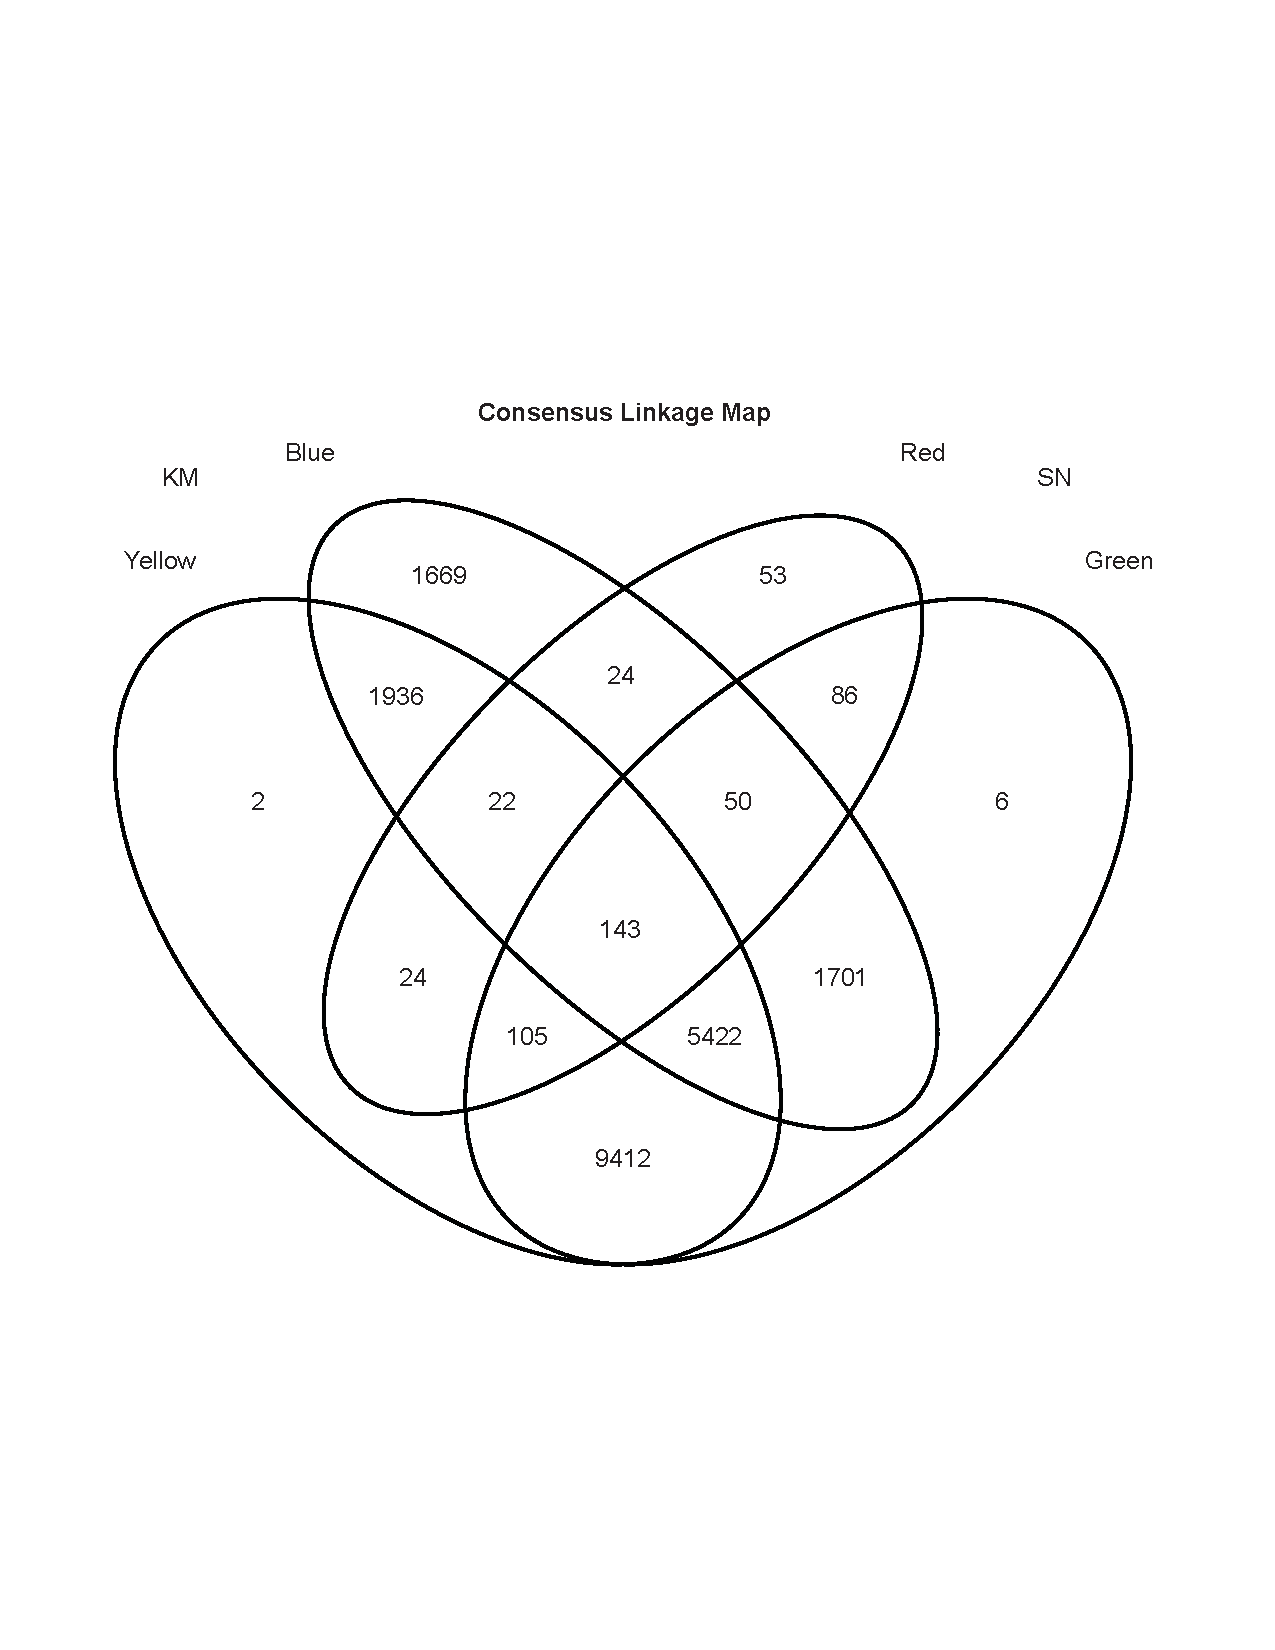
\includegraphics[width=1.0\textwidth]{Figure02_TGG}
  \caption{Sharing of contigs across maternal tree maps from which the consensus map was constructed. Counts in each cell
  represent the number of unique contigs appearing on the final consensus map. KM = Klamath Mountains; SN = Sierra Nevada.}
  \label{f:Figure02_TGG}
\end{figure}
 

\begin{figure}[ht]
  \centering
  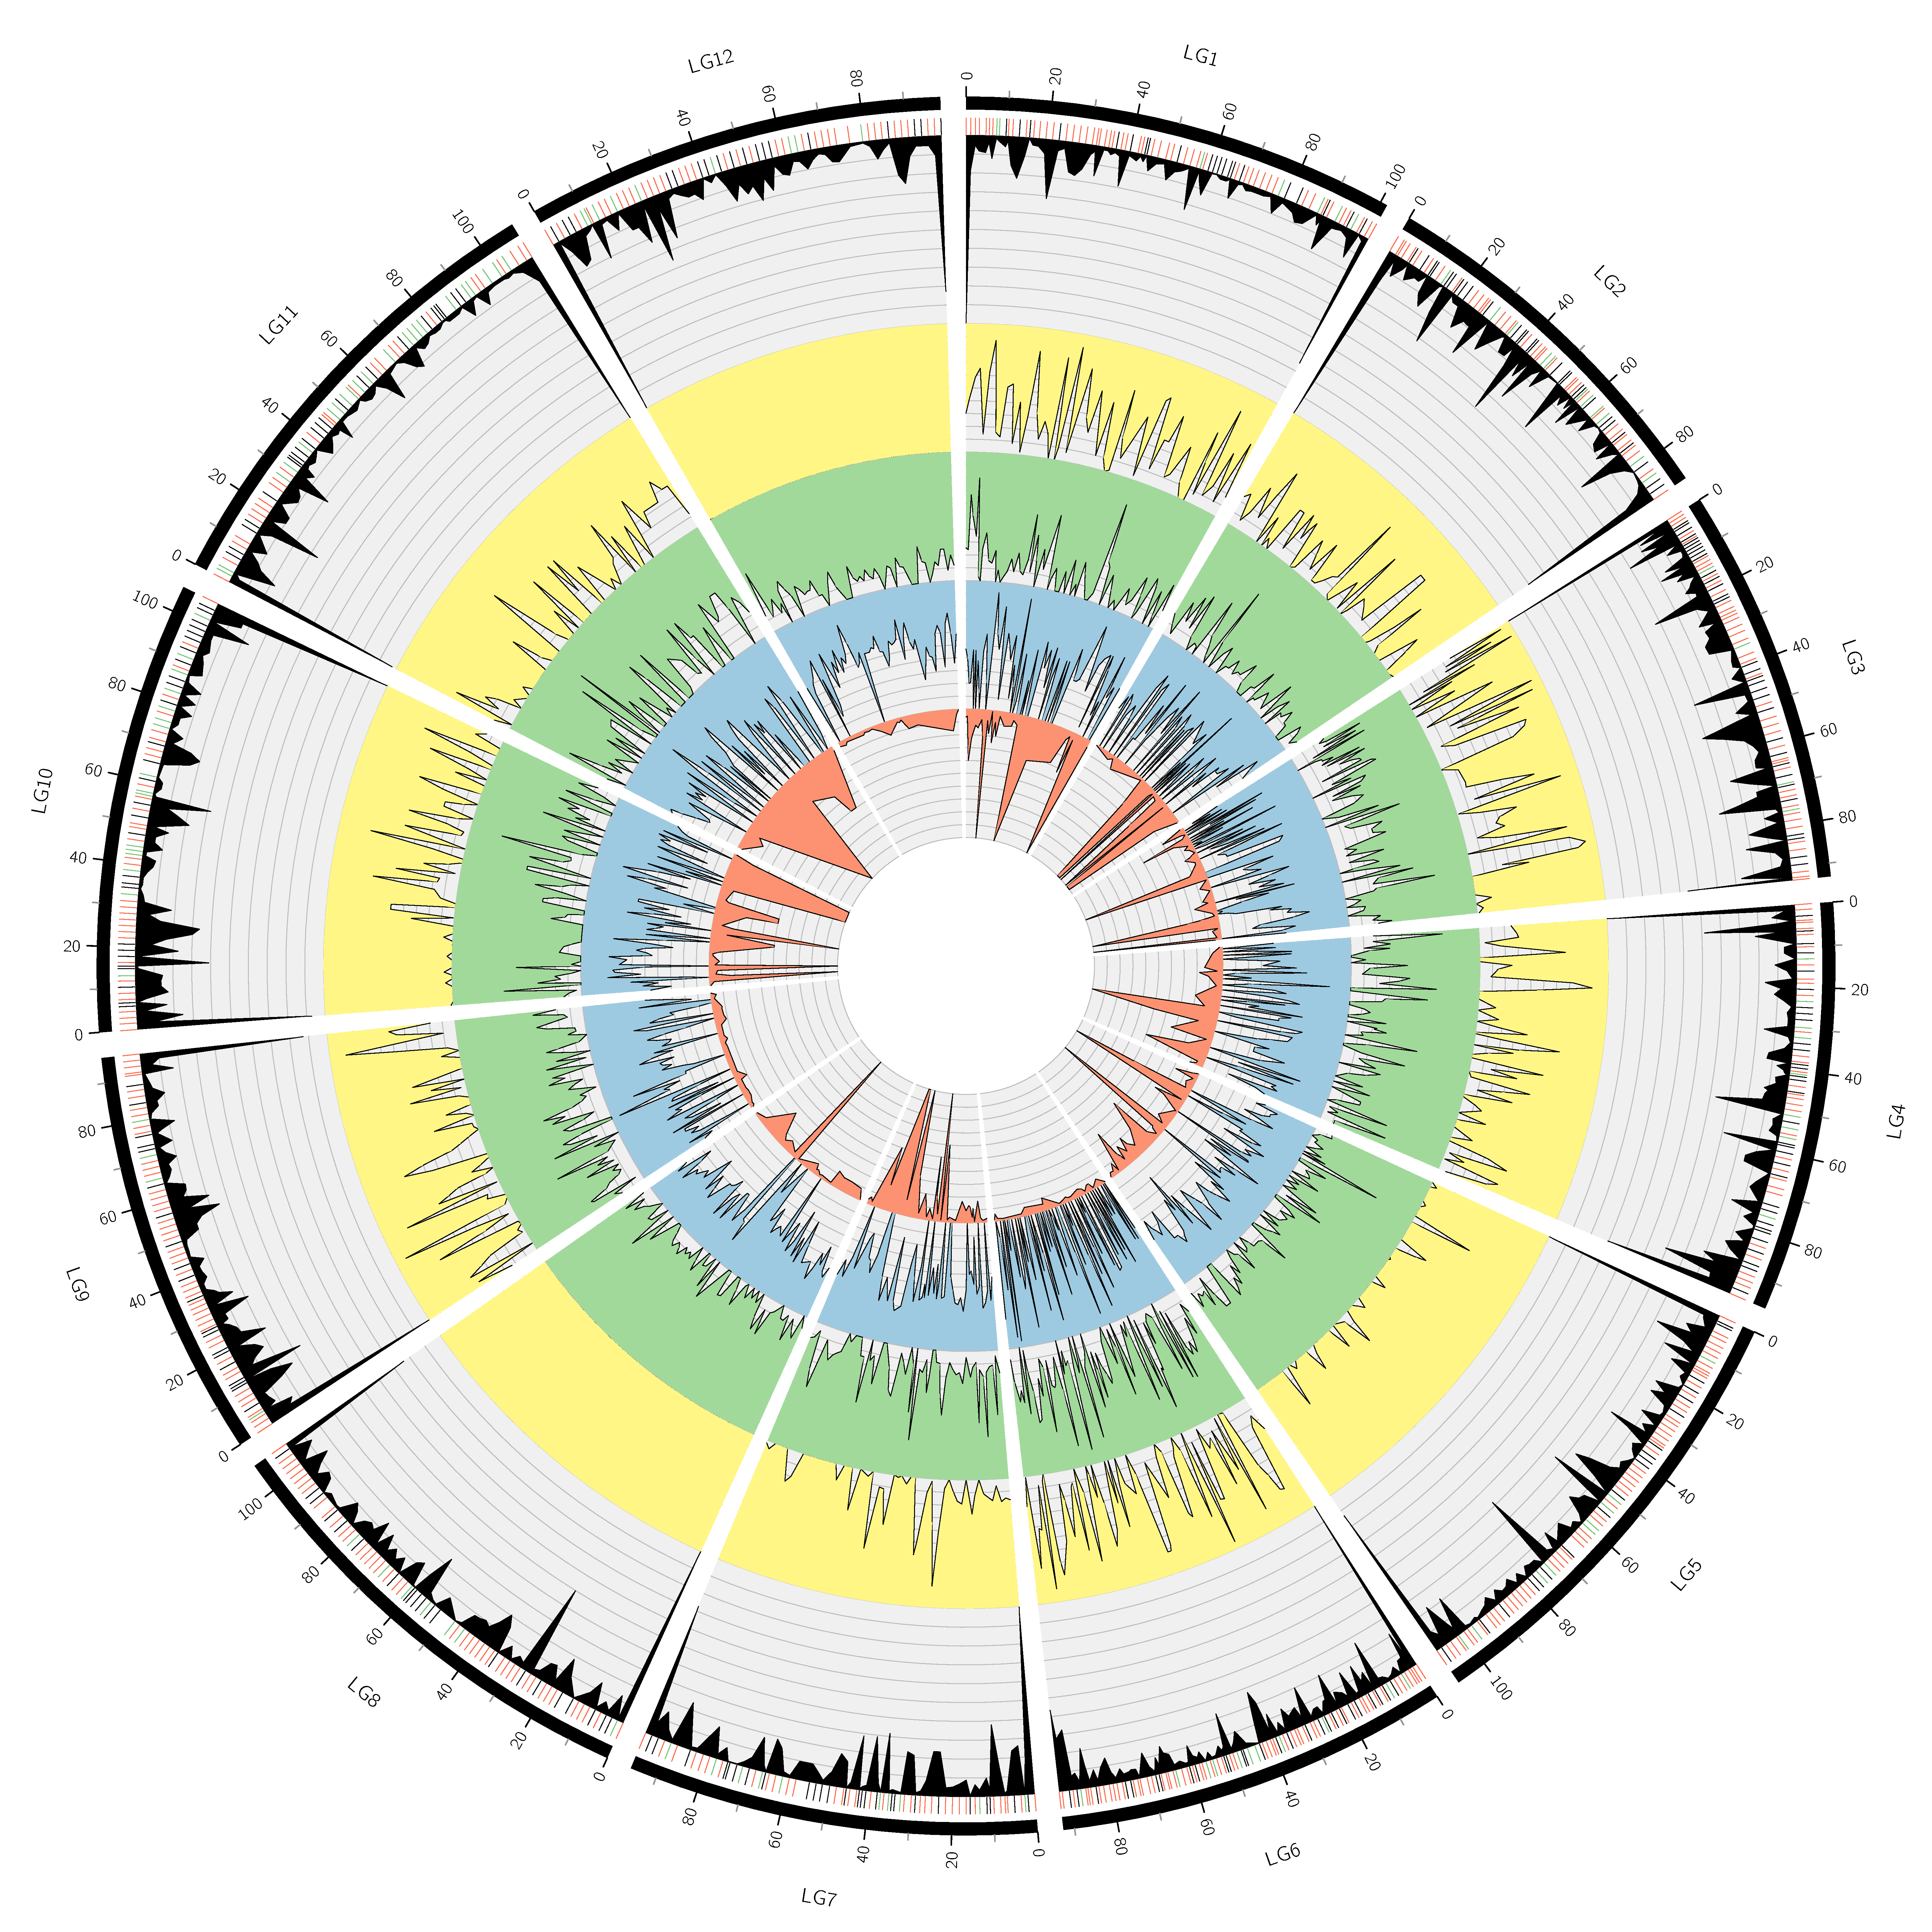
\includegraphics[width=\textwidth]{circos_con}
  \caption{Consensus linkage map.  Positions on each linkage group are in centiMorgan. The color of the bars indicate SNP
annotation density at each position ($\ge 50\%$ = green, $\ge 25\%$= red, $< 25\%$ = black). Density of SNPs (count of SNPs mapping 
to a specific position on the linkage group) at each position are indicated by histograms. The total density at each position is indicated 
in black, and density by family is indicated by respective color.}
  \label{f:con}
\end{figure}

\clearpage

\beginsupplement

\section*{Supplementary Materials}

%put supplementary figures and tables below here
\subsection*{Supplementary Text}\label{ss:supp}

A nonparametric permutation analysis was used to test the hypothesis that sharing of polymorphic
contigs was greater between maternal trees located in the same regional population. The null hypothesis
in this case is that the degree of sharing between trees in the same regional population is not different
than between trees in different regional populations. To conduct this test, we constructed a null distribution 
of the difference between mean within versus mean between levels of contig sharing. This distribution was
based on permutations, where each permutation consisted of randomly sampling with replacement contigs from the full set
of contigs prior to filtering for each maternal tree identifier. The number of each contigs for each maternal
tree identifier was equal to that observed in the original dataset. Given these assignments, the degree of sharing (DS)
between trees was calculated as:

DS = number of contigs shared/number of unique contigs in the pairwise comparison

Given four maternal trees, there are 6 pairwise comparisons, of which there are 2 within regional population and
4 between regional population comparisons. Using these pairwise values, we constructed a test statistic defined as
the difference between the mean within regional population value of DS and the mean between regional population
value of DS. We simulated $10000$ value of this test statistic to form the null distribution and rejected
the null hypothesis when the observed test statistic fell in the upper 95\% tail of this null
distribution. Using this approach, the observed test statistic was 0.06337814. The limits of the simulated null distribution
were -0.0349 to 0.0415. Thus the observed test statistic fell completely outside the upper tail of the null distribution, which
gives a \textit{P}-value of $P < 0.0001$.

The spatial distribution of contigs along linkage groups was tested against complete spatial randomness using simulations.
Specifically, we used the variance in the observed number of contigs mapped to each unique position across the entire linkage map
as the test statistic. The null distribution of the test statistic was created by simulating $10000$ Poisson-distributed variables, each 
with the number of random values equal to the number of unique positions on the linkage map under consideration and the mean 
equal to the mean number of contigs per position. For each Poisson-distributed variable, the variance was calculated. The set of
$10000$ variances was used as the null distribution expected under complete spatial randomness. A separate null distribution was
constructed for each maternal tree. If the observed variance fell in either the 2.5\% or 97.5\% tail of the null distribution, the null
hypothesis was rejected. For example, the values used 
for the consensus linkage map were: observed variance $= 1245.423$, average expected variance of Poisson-distributed variable $= 
23$, $95\%$ CI of null expectation: $20.915 - 25.246$, and limits of the null distribution: $19.214 - 27.655$.The \textit{P}-value for
the observed variance is thus $P < 0.0001$. This test does not explicitly test spatial randomness of the unique positions on a linkage
map, but rather tests the assumption that the intensities (i.e., the number of mapped contigs) at each position follow a Poisson distribution. 
This approach was chosen because distances in the inferred linkage maps were sensitive the error correction and imputation. Of course, 
the number of contigs at each mapped position is also sensitive to this process, although relaxing the error correction parameter in
Maskov resulted in similar results for a range of values that resulted in realistic linkage map lengths. Thus, we were confident that this
result is not only a function of error correction and imputation. All linkage maps except for the single-tree map from the red maternal tree
had greater than expected variances across positions in counts of mapped contigs relative to the null model of a Poisson-distributed variable.

\subsection*{Supplementary Tables}\label{ss:supp}


\subsection*{Supplementary Figures}\label{ss:supp}




\end{document}
